\begin{figure*}[!ht]
\centering
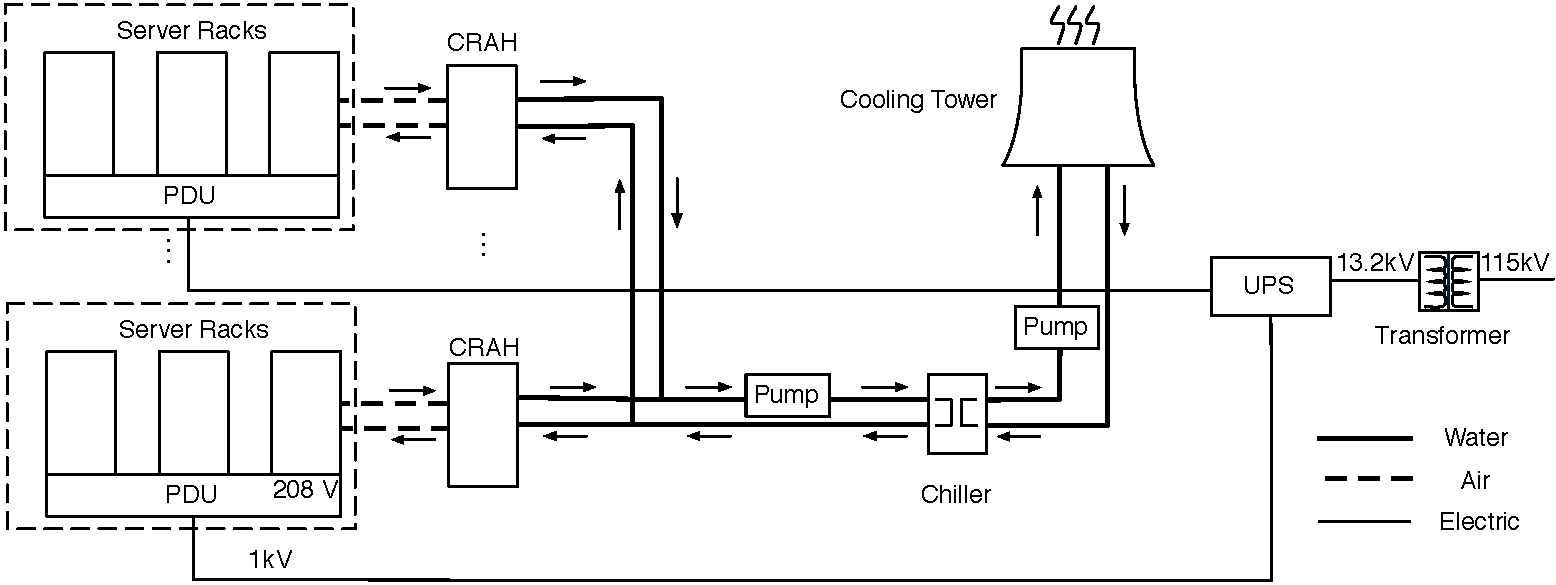
\includegraphics[width = 6.5 in]{Appendices/WEED/figure/HeatFlow.pdf}
\caption{ \textbf{Power and Cooling Flow.} }
\label{figure::PowerFlow}
\vspace{-.1 in}
\end{figure*}

\section{Related Work}

%{\bf Modeling system power}

The literature on computer system power management is vast; a recent survey appears in \cite{KaxirasBook08}.  A tutorial on data center infrastructure and related research issues is available in \cite{BarrosoBook09}.  

Numerous academic studies and industrial whitepapers describe or apply models of power draw for individual data center subsystems.  Prior modeling efforts indicate that server power varies roughly linearly in CPU utilization \cite{Fan07,Rivoire08}. Losses in power conditioning systems and the impact of power overprovisioning are described in \cite{Fan07, Rasmussen113}. Our prior work proposes mechanisms to eliminate idle power waste in servers \cite{Meisner09}.  Other studies have focused on understanding the thermal implications of data center design  \cite{Heath06, Patel02}.  Power- and cooling-aware scheduling and load balancing can mitigate data center cooling costs  \cite{Moore06, Parolini08}.  Though each of these studies examines particular aspects of data center design, none of these present a comprehensive model for total data center power draw.  

%{\bf Modeling thermal}



